%----------------------------------------------------------------------------------------
%	PACKAGES AND OTHER DOCUMENT CONFIGURATIONS
%----------------------------------------------------------------------------------------

\documentclass[paper=a4, fontsize=11pt]{scrartcl} % A4 paper and 11pt font size
\usepackage{multicol}
\usepackage[T1]{fontenc} % Use 8-bit encoding that has 256 glyphs
\usepackage{fourier} % Use the Adobe Utopia font for the document - comment this line to return to the LaTeX default
\usepackage[english]{babel} % English language/hyphenation
\usepackage{amsmath,amsfonts,amsthm} % Math packages
\usepackage{listings}
\usepackage{lipsum} % Used for inserting dummy 'Lorem ipsum' text into the template
\usepackage{graphicx}
\usepackage{subfig}
\usepackage{float}

\usepackage{sectsty} % Allows customizing section commands
\allsectionsfont{\centering \normalfont\scshape} % Make all sections centered, the default font and small caps

\usepackage{fancyhdr} % Custom headers and footers
\pagestyle{fancyplain} % Makes all pages in the document conform to the custom headers and footers
\fancyhead{} % No page header - if you want one, create it in the same way as the footers below
\fancyfoot[L]{} % Empty left footer
\fancyfoot[C]{} % Empty center footer
\fancyfoot[R]{\thepage} % Page numbering for right footer
\renewcommand{\headrulewidth}{0pt} % Remove header underlines
\renewcommand{\footrulewidth}{0pt} % Remove footer underlines
\setlength{\headheight}{13.6pt} % Customize the height of the header

%\numberwithin{equation}{section} % Number equations within sections (i.e. 1.1, 1.2, 2.1, 2.2 instead of 1, 2, 3, 4)
%\numberwithin{figure}{section} % Number figures within sections (i.e. 1.1, 1.2, 2.1, 2.2 instead of 1, 2, 3, 4)
%\numberwithin{table}{section} % Number tables within sections (i.e. 1.1, 1.2, 2.1, 2.2 instead of 1, 2, 3, 4)

%\setlength\parindent{0pt} % Removes all indentation from paragraphs - comment this line for an assignment with lots of text

%----------------------------------------------------------------------------------------
%	TITLE SECTION
%----------------------------------------------------------------------------------------

\newcommand{\horrule}[1]{\rule{\linewidth}{#1}} % Create horizontal rule command with 1 argument of height

\title{	
\normalfont \normalsize 
\textsc{Syddansk Universitet} \\ [25pt] 
\horrule{0.5pt} \\[0.4cm] % Thin top horizontal rule
\huge Clustering \\ % The assignment title
\horrule{2pt} \\[0.5cm] % Thick bottom horizontal rule
}

\author{Bjarki Sigurdsson \\ Abdulrahman Abdulrahim \\ Miguel de la Colina \\ Group 5}
 % Your name

\date{\normalsize\today} % Today's date or a custom date

\begin{document}

\maketitle % Print the title

%----------------------------------------------------------------------------------------
%	PROBLEM 1
%----------------------------------------------------------------------------------------


\section*{Abstract}

\paragraph{The purpose of the exercise was to use clustering to see how this would affect the performance on the knn classification but now taking into consideration the centroid of the clusters also creating dendograms to get a visual representation of how this clusters are made and run evaluation methods to see how well they are performing.}
%The purpose of this report is to use the k-nearest neighbor algorithm on a data-set made of ciphers. We will be dividing the data into two sets, one for training and one for testing. We will analyze the results for different values of k and DPI to see how this alters our results. Also we will be applying the  Gaussian smoothing with various sigmas in order to see how does this alter the results.}  

%------------------------------------------------


%----------------------------------------------------------------------------------------
%	PROBLEM 2
%----------------------------------------------------------------------------------------

\section{Kmeans clustering}
For this part of the exercise we will try to improve the performance by performing kmeans in each cipher individually for the training set in order to represent them as cluster centroids and then perform knn using the centroids we have obtained. \\

We will be training the kmeans algorithm using different sizes of clusters ( 25, 50, 100, 200) to see how the accuracy  will change in bot the person-dependent and person-independent set. 

\begin{table}[h]
\centering
\caption{Accuracy Results.}
\label{tab:pca}
\begin{tabular}{|c|r|r|r|}
\hline
clusters & p-dependent accuracy & p-independent accuracy  \\ \hline
25    & .83875              & .14025                   \\
50    & .87              & .143                       \\
100   & .87675             & .149                        \\
200    & .89275             & .17225                 \\
\\ \hline
\end{tabular}
\end{table}

\begin{figure}[h]
	\centering
	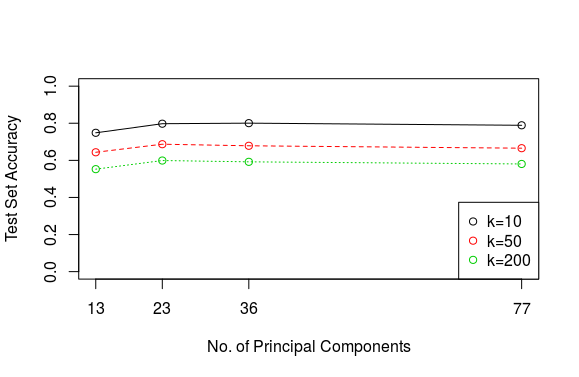
\includegraphics[width=0.8\textwidth]{../../accuracy.png}
	\caption{Accuracy graph for dependent and independent data-sets.}
	\label{fig:scree}
\end{figure}


As we can see from the results that we received from table 1 we can see that the accuracy level actually increases as we increase clusters which makes sense seeing that as we begin creating more clusters we are being more specific to finding to which cluster they belong giving us a more accurate result than doing it with a fewer number of clusters.\\

In figure one we can see how the accuracy varies for each of the data sets depending on how many clusters we are using and here it is easier to see how the accuracy does increase even if it's a little while we increment the number of clusters.


\clearpage
\section{Hierarchical Clustering}
A dendogram is a tree diagram that will show how the clusters have been made so that we can see the relationships we have with each of the ciphers here we will see how this relationships look and how they relate with the cross validation tables from knn.\\

If we look at figure 4 and figure 5 we can see that there is a relation between both of them we can se that there are some clusters that actually are matched with different numbers at lower levels like with 7 and 1, and if we look at 7 and 1 in the cross validation table we can actually see that 1 and 7 have a number of misplaced results where the 1 is mistaken for a 7 which actually explains why we could be seeing this types of clusters at lower levels.

\begin{figure}[h]
	\centering
	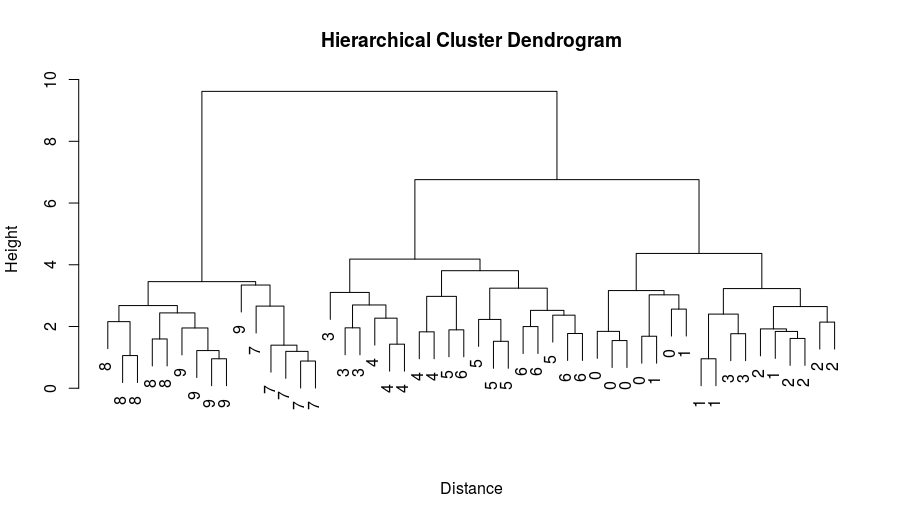
\includegraphics[width=0.8\textwidth]{../../dendrogram.png}
	\caption{Low level dendogram containing 5 instances of each digit.}
	\label{fig:scree}
\end{figure}

\begin{figure}[h]
	\centering
	\includegraphics[width=0.8\textwidth]{../../clustering.png}
	\caption{kmeans clustering.}
	\label{fig:scree}
\end{figure}

\begin{figure}[h]
	\centering
	\includegraphics[width=0.8\textwidth]{../../downsampling.png}
	\caption{Random down sampling.}
	\label{fig:scree}
\end{figure}
\begin{figure}[h]
	\centering
	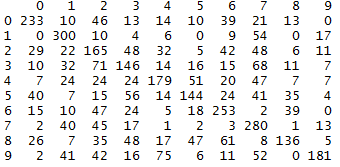
\includegraphics[width=0.8\textwidth]{../../confusionMatrix.png}
	\caption{cross validation table knn.}
	\label{fig:scree}
\end{figure}


%We see that the results are near-identical. This is logical as PCA depends on the eigenvalue decomposition of the covariance matrix and is therefore not significantly altered by normalization via robust methods.



%We will be using R which is a statistical language in order to test the k-nearest neighbor algorithm, firstly we will have to generate our data-sets which are taken from scanned ciphers and loaded through the function \texttt{loadSinglePersonsData}, once the data is loaded we shuffle the data with a seed for reproducible results. With this done we split the data into test and train so that we are able to test the data after we have trained and be able to use different data from the one that was trained.



\begin{flushleft}
%For this test we will be varying the number of k to see how the result actually varies when we begin to change it's value we will check how the speed and test recognition are affected by this change. This is to see how important really is to select the correct k and to see if having selected the wrong one could affect your results substantially.
\end{flushleft}

\begin{flushleft}
%We will also be doing cross validation of the results in order to see if the results of the trained model will fit for other hypothetical, set of data this will be done by running 10 times a 90\%/10\% split of the data-set. The pseudocode for the cross-validation is shown below.
\end{flushleft}

\begin{flushleft}
%Finally after testing it with the smoothing implementation that was in \texttt{loadImage.r} we have to implement the smoothing using a different method. We used the Gaussian smoothing  with various sigmas, this is implemented in the EBImage package as \texttt{gblur()} which receives as parameter the image and the sigma.   
\end{flushleft}
%------------------------------------------------


%----------------------------------------------------------------------------------------


%We see that the accuracy does vary with k. Notably, k=1 results in a perfect fit for the training set but this will often, in theory, result in overfitting of the data. Thus we use the rule of thumb of taking the square root of the sample size as the k and approximate it to k=50 for further testing.\\

%Though the timing measurements presented in the table are quite noisy, we see that the computation time seems to increase with DPI. This is logical as the number of pixels in the images has a square relationship to the DPI. Below we will present more accurate timing measurements and discuss their dependence on k.\\

%For more accurate timing measurements, we ran the \texttt{knn()} function repeatedly for k=1 and k=100 and compared the results. for DPI=300, we obtained mean computation times of 3.98s and 4.75s for k=1 and k=100, respectively. This is to be expected as for larger k, each point needs to be checked against more neighbours, resulting in more computations.\\

%We performed cross-validation on the data with our chosen k for varying DPI values. In general, we found the accuracy of the kNN algorithm to be independent on the image quality, at least for the DPI values tested. Thus only results for DPI=100 are shown below. We obtained a mean accuracy of 0.880 with a standard deviation of 0.056.\\


%For our tests with image preprocessing we obtained the results shown below for different sigmas in the gaussian low-pass smoothing filter. We see that the smoothing seems to increase the accuracy of the algorithm to some degree.\\


%Finally we ran the first test on the entire data set. Cross-validation as well as accurate timing was not performed for this part due to a lack of computation power. This was also the reason we only tested with k=50. k=200 may have been more accurate as the data set was 18 times larger than in previous parts.\\

%We obtained accuracy results of 0.9954 on the training set and 0.9949 on the test set. We timed the execution time of the \texttt{knn()} function and found it to be 20 minutes and 35 seconds. From these results, in comparison to the previous, one can argue that the benefit of having a larger data set is greater than the variance introduced by different handwritings. Moreover, the variance in handwriting in the data may even be beneficial to the accuracy of the algorithm.\\
\clearpage
\section{Evaluation methods}
As we can see in figure 6 the precision recall curve shows that if we have low recall we will be having a high level of precision and as the recall begins to increase we will start to see how the precision decreases and although with each k the curve varies we can still see that all of them follow similar behaviors.

Now in figure 7 we have a graph which displays the F1-score (which takes into account both the precision and the recall) against the number of clusters we have decided to use and as we can see the F1-score begins to decrease noticeably as the number of clusters starts to increase.
\begin{figure}[h]
	\centering
	\includegraphics[width=0.8\textwidth]{../../PRcurve.png}
	\caption{Precision-Recall curve.}
	\label{fig:scree}
\end{figure}
\begin{figure}[h]
	\centering
	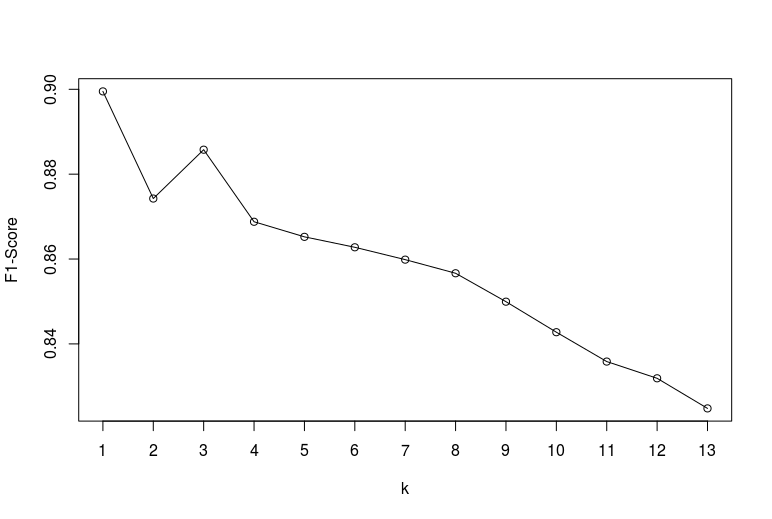
\includegraphics[width=0.8\textwidth]{../../f1score.png}
	\caption{F1 score vs k graph.}
	\label{fig:scree}
\end{figure}



%--------------------------------------------------

\end{document}
\grid
